%********** Chapter 1 **********
\chapter{System Analysis and Design}

In this chapter we explain the system requirements, we also provide an analysis of the system architecture along with a description of each module.

\section{System Requirements}

Our system should build a 3D model of an indoor environment scanned by a user holding Kinect camera, the system must work in real-time meaning that the model will be constructed while the user is scanning the environment, this will help the user see what parts of the environment are missing and identify any mistakes if any.

Our main focus in this system is for it to be available for ordinary users that may not have access to expensive hardware and may not be experienced in 3D scanning. For this reason, we used techniques that give good results while not needing much processing, we also handle any mistakes commited by users while moving the Kinect such as moving fast.

To prove the usefulness of the system, we enable the user to do simple editing on the constructed model, this simple editing includes moving and deleting some objects from the scene.
\pagebreak

\section{Main pipeline and architecture}

SLAM systems can be described as iterative systems as the second frame is aligned to the first frame, then the operation is repeated for each new frame.

We explain briefly the main steps of the pipeline, each step is explained in more details in following chapters:

\subsection{Frame Acquisition}
   We use the OpenNI library to obtain the current viewed scene by Kinect, this scene is represented as a 3D point cloud, for each point we have the $x, y and  z$ coordinates in meters along with the RGB components of the pixel color.
   The captured point cloud is then converted into two images; one representing the colored scene and another containing the depth information for each pixel, this step is done so that we can use these images later for feature tracking.

\subsection{Feature Tracking}
   To align any two consecutive frames, we need to obtain the transformation between between the two frames, this can be achieved by tracking feature points from one frame to another, then use transformation calculations to obtain the best transformation between the two set of points.
   In chapter 5 we talk in details about two different methods for feature tracking and compare their results.

\subsection{Transformation Calculation}
   After having two sets of correspondence between the two consecutive frames, we calculate the transformation using both closed form method known as Horn's method followed by Iterative Closes Point procedure to enhance the results and get a more accurate transformation.

\subsection{Concatenation and Presenting Results}
   Having obtained the required transformation between the two frames, the second is transformed and concatenated to the global point cloud that is viewed by the user.
   The results of construction can be also saved using the popular .ply format as a mesh or a point cloud.

\subsection{Loop Closure and Global Optimization}
   At the end of the scanning operation, it is likely that the user will return to the starting point, theoritcally the first and last frames should concide over each other, but due to both cumulative errors in alignment and numerical errors the alignment of the first and last frame will not be exact, so we need to detect a loop in the scanning and try to make optimize the global scene to distribute the error.
\pagebreak

The following figure summarizes the general pipeline:
\begin{figure}[H]
\centering
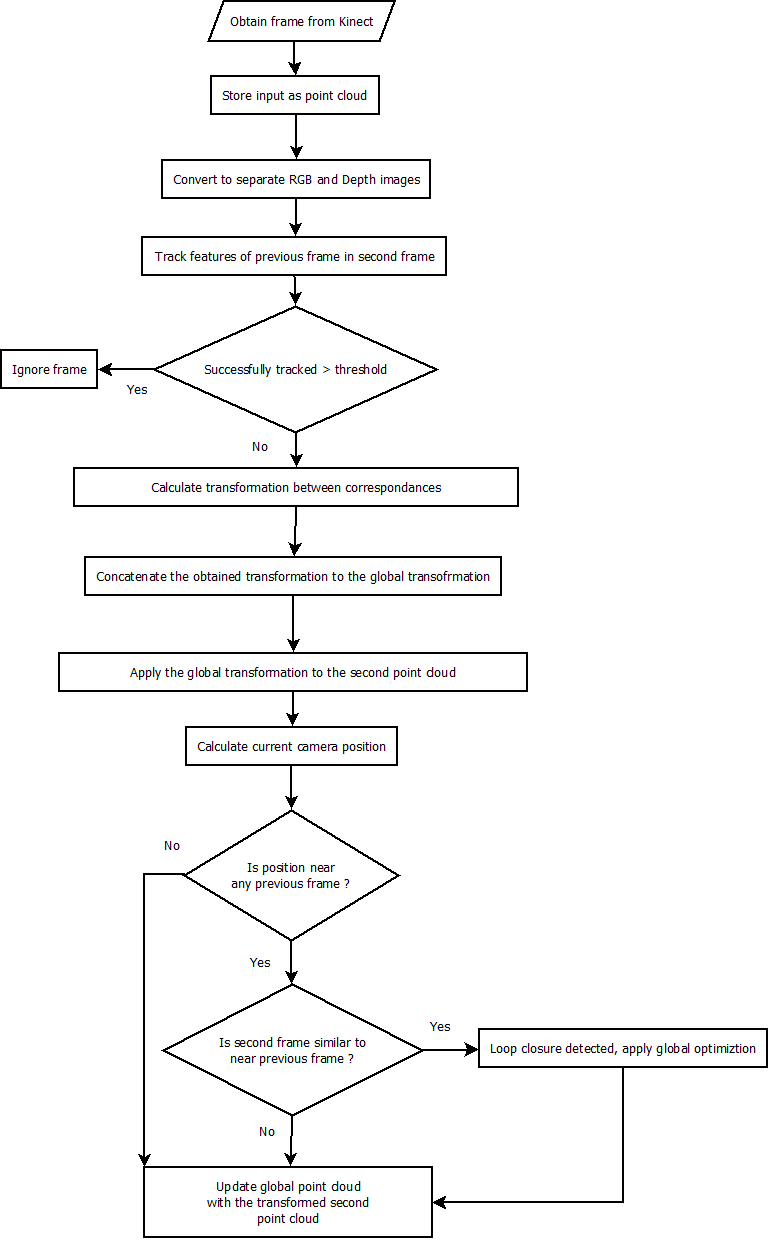
\includegraphics[scale=0.45,keepaspectratio=true]{System_Analysis_and_Design/pipeline.png}
\caption{System Pipeline}
\label{fig:system_pipeline}
\end{figure}

\section{System components}

We divide our system to a number of components, each component is responsible for doing only one function, we tried to make the design as cohesive as possible and reduce the coupling between components as possible.

Each component is implemented in a class that offers methods that are used by other components, here is a list of classes and their descriptions:

\begin{itemize}
  \item Transformation: a data class that represents a 3D transformation
  \item HornMethod: this class contains the code needed to calculate the best transformation between two sets of 3D points
  \item Tracker: this class provides feature tracking using optical flow and 	SURF feature detection and matching
  \item Alignment: this class has functions that uses the previous components to obtain an initial transformation
  \item SurfaceConstruction:
  \item Segmentation:

\end{itemize}

\begin{figure}[H]
\centering
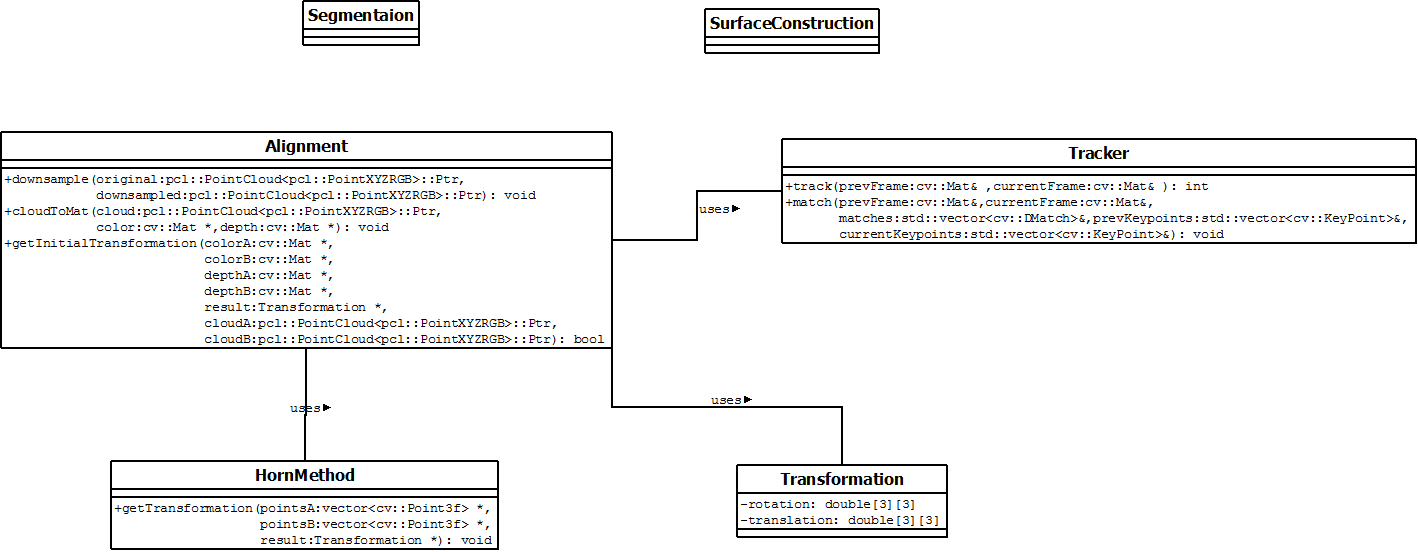
\includegraphics[width=150mm,height=150mm]{System_Analysis_and_Design/class_diagram.png}
\caption{Class Diagram}
\label{fig:class_diagram}
\end{figure}

\subsection{Libraries and tools}
